% !TEX root = ../main.tex
\section{Data Collection}\label{sec:datacollection}

	%Hvorfor valgte jeg en teknisk løsning og ikke penn og papir eller andre metoder??
	\subsection{Review of Human Properties}

      % - Hvilke kan brukes?
      % - Hvilke ble tatt med?
      % - Hvorfor ble de tatt med? Evt ikke tatt med?
      % Alle sier noe om hvem en person er, noen er mer fysiske egenskaper mens andre er ren bakgrunnsinformasjon. 
      
     	\subsection*{Age} 
      A group of people within a particular group of age may have different risk awareness. A person with an age of 30-40 and an individual with an age below 20 may have different concerns with security. An individual in the age between 30-40 may use their phone to perform a task with requiring high security. A person with an age below 20 may not have the same security awareness because of the different use of mobile devices. Age is also interesting demographic information that can be used to group the respondents into different subgroups.

      \subsection*{Gender} 
      Psychological studies have reported that males are more likely to take risks than females \cite{Byrnes}. In the literature review, there was no reported results found in genders risk awareness in information security, nor people's choice of patterns based on gender.

      \subsection*{Nationality} 
      The nationality of users is often used in research on graphical passwords. When asking a person about their PIN code, a nationality can be used to find likely numbers to appear because some cultures associates a number with a historical or religious event. In a research on the ``PassFace'', the nationality of the participants was proven to be valuable because people tended to choose faces from the same race and nationality. In this research, it is uncertain how much this information will help to prove any connection between nationality and users choice in patterns. Properties like language preference and reading/writing orientation look more promising for this research.

      \subsection*{Language preference} By asking the respondent about their language preference, this can be used to see if the way they write or the alphabet they use impacts their choice in lock pattern. For example, the Chinese words are written in a different way then people using the Latin alphabet. In the Android Unlock Patterns, people are able to create patterns looking the same as the letters ``L'', ``M'', and ``O''. The Figure~\ref{fig:letters2} there is an illustration the letters that are possible to select as a lock pattern. The same possibility could might be found in languages using a different alphabet than the Latin. When looking at PIN codes, there are certain numbers that have a different meaning than only its numeric value. In China, people are associating certain words with numbers or things based on the similarities of sound. For example, the number eight is considered as a lucky number because it is pronounced ``ba'', which sounds like the Chinese word for prosperity. When studying other numbers we can map the number 4 to ``death'', and the number 775 is decoded to ``Kiss me'' \cite{ChineseChatCodes}. Looking at selection of PIN codes based on people's language is an interesting. People tend to choose numbers in PIN codes that they can associate the number with something they now, like their date of birth. There is not known if the same observation can be found in the selection of patterns, but the language preference might give some interesting results.

        \begin{figure}[H]
          \centering
          \subfigure[The letter L]{
            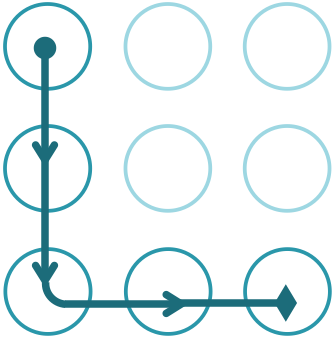
\includegraphics[width=0.25\textwidth]{pics/letters/bokstavenL.png}
          }
          \vspace{0.2cm}
          \subfigure[The letter M]{
            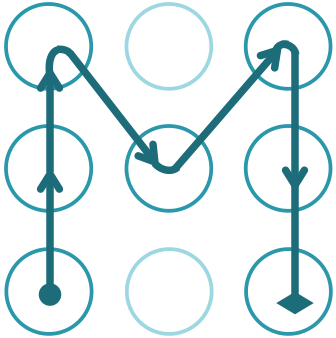
\includegraphics[width=0.25\textwidth]{pics/letters/bokstavenM.png}
          }
          \vspace{0.2cm}
          \subfigure[The letter O]{
            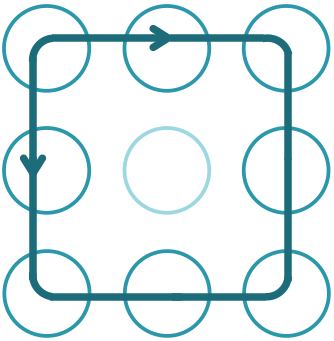
\includegraphics[width=0.25\textwidth]{pics/letters/bokstavenO.png}
          }
          \caption{Patterns corresponding to letters}
          \label{fig:letters2}
        \end{figure}

      \subsection*{Occupation}
      This information is valuable information due to the knowledge level of the respondents. The occupation of the a respondent is simply if a person is a student, employed, not employed or retired.

      \subsection*{Profession}
      The profession of a person may say something about a persons knowledge and background. When looking at profession, a person with a profession in IT may be more certain of the security aspects than people in other professions. It may cause bias in the data if people with enough knowledge of security overcompensate their choice of lock pattern because they want to prove their knowledge.  

      \subsection*{Handedness}
      An interesting property of humans is the fact that people write with either left or right hand (and sometimes both). This property can influence the way a person are holding a mobile phone, and may impact the way that a person is choosing their pattern. In the literature review, it was not found any studies that reported results of people choices in patterns based on the hand used. Published research \cite{Uellenbeck} found that over 40\% of the participants in their study started their Android pattern by beginning in the top left corner, but did not record the hand used when making the pattern. My hypothesis is that a left handed person may be using the left hand while interacting with the phone, making the probability for starting in the right upper corner bigger. This property has never been used before in analyzing Unlock Patterns. In Figure~\ref{fig:handedness} it is illustrated handedness and likely starting point. The numbers are collected from the research by Uellenbeck \cite{Uellenbeck}, where they measured likely initial points. Since it is more likely that people are right-handed, are we able to mirror the results to left-handed people? My hypothesis as stated earlier is that people that are left-handed are more likely to start in the upper right corner, while people that are right-handed are more likely to start in the upper left corner. The percent attached to the node are indicating the probability for starting the pattern at that node. 

        \begin{figure}[H]
          \centering
          \subfigure{
            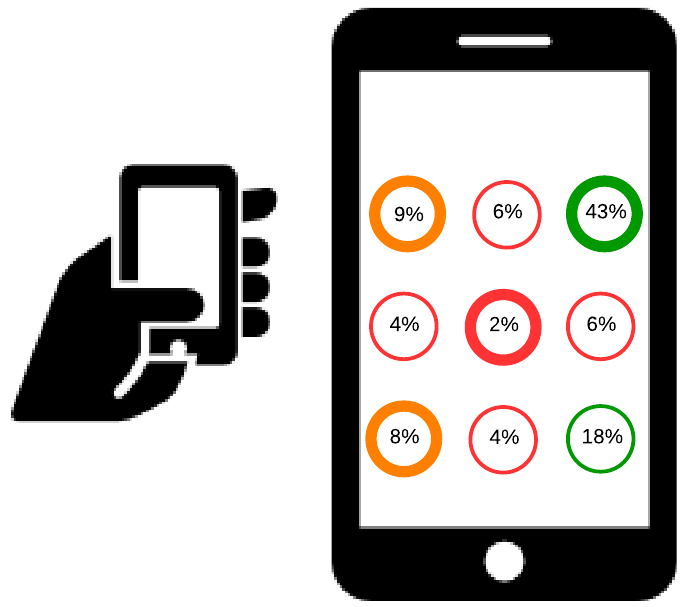
\includegraphics[scale=0.2]{pics/review/handednessLeft.png}
          }
          \subfigure{
            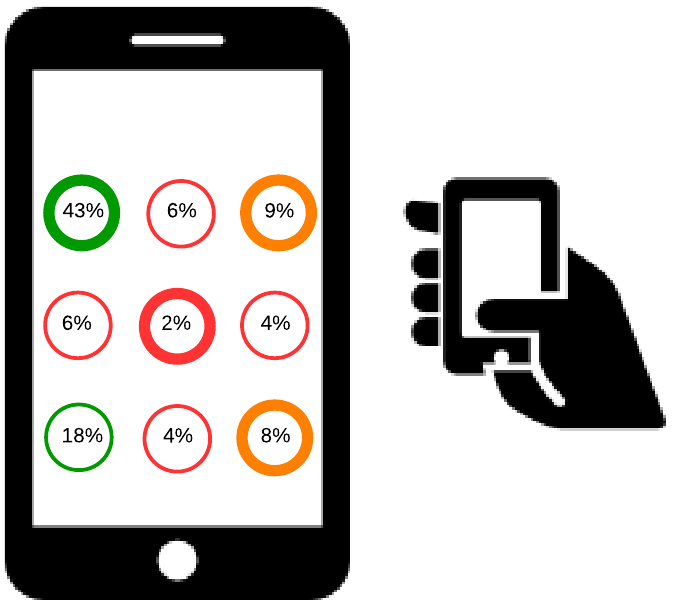
\includegraphics[scale=0.2]{pics/review/handednessRight.png}
          }
          \caption[Likely chosen initial starting point and handedness]{Likely chosen initial starting point \cite{Uellenbeck} and handedness}
          \label{fig:handedness}
        \end{figure}

      \subsection*{Reading and writing orientation}
      In different cultures, there is a difference in the reading and writing orientation. Cultures of Europe and America are usually writing and reading horizontally from left to right, but there are other cultures that do otherwise (Figure~\ref{fig:orientation}). Traditionally, Chinese, Japanese, and Korean are writing text vertically in columns from top to bottom, from right to left. Another writing orientation is horizontal from right to left that are used in Arabic cultures. Today, the vertical orientation from top to bottom is often in a horizontal way due to the influence of English and the increased computerized typesetting, but both ways are still in use. There are research that have reported that the writing orientation are affecting the visual attention and memory \cite{Chan}. They found that the reading orientation affected the way a person would memorize objects. They reported that English and Chinese speakers tended to remember an image that appeared in the top, left-hand side of the screen and the Taiwanese speakers tended to remember the images in the upper right-hand side of the screen. An interesting aspect of the reading and writing orientation is to see if people from different cultures are choosing different patterns due to their writing orientation. 

        \begin{figure}[H]
          \centering
          \subfigure[Left-to-right]{
            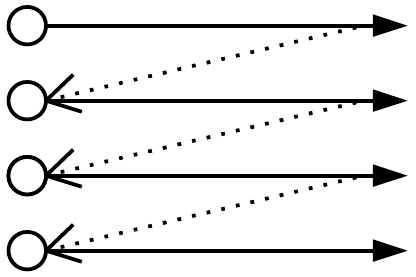
\includegraphics[scale=0.25]{pics/review/leftright.png}
          }
          \subfigure[Right-to-left]{
            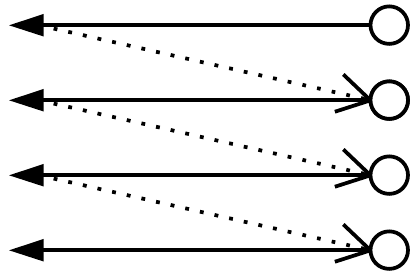
\includegraphics[scale=0.25]{pics/review/rightleft.png}
          }
          \subfigure[Top-to-bottom, left-to-right]{
            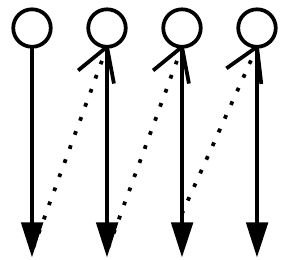
\includegraphics[scale=0.27]{pics/review/topbottom.png}
          }
          \caption{Reading and writing orientation}
          \label{fig:orientation}
        \end{figure}

      \subsection*{Handsize}
      Smartphones today tends to get bigger and bigger in size. An interesting analysis could be done by looking at user's choice in patterns based on size of their hands and size of mobile phone where a pattern is made. By looking at a situation where a person with a small hand is interacting with a big screen, it may be hard to reach certain areas of the screen when holding the smartphone in one hand. Maybe a right-handed person with a small hand interacting with a large screen will not be able to reach the upper left corner? (Illustrated in Figure~\ref{fig:reachablePoints}).

        \begin{figure}[H]
          \centering
          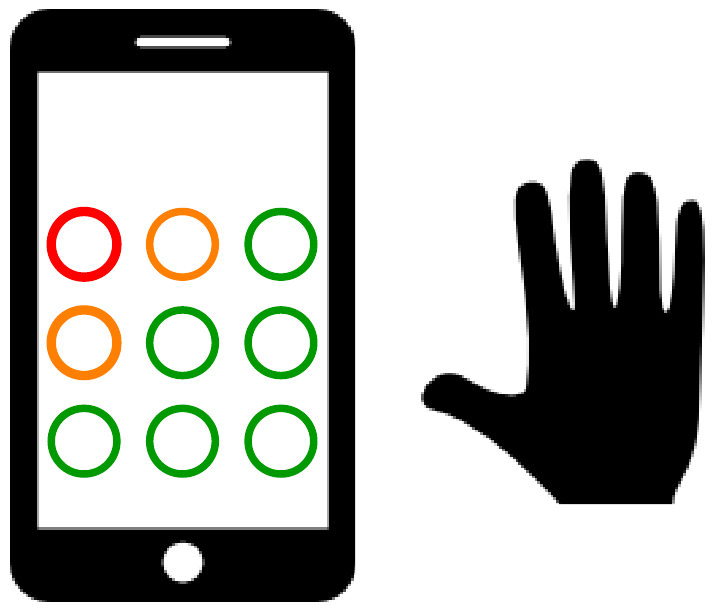
\includegraphics[scale=0.22]{pics/review/screenHand.png}
          \caption{Reachable points on screen}
          \label{fig:reachablePoints}
        \end{figure}

      \subsection*{Finger used when creating pattern}
      When looking at the finger used when creating the pattern, it impacts the areas on the smartphone where a person can reach. When interacting with a smartphone, the most common way is to either use the thumb or the forefinger. When combining this property with the screen size and the size of the hand, we might be able to predict selection of patterns and eliminate some possibilities. In a book called ``Designing Mobile Interfaces'' \cite{Hoober}, they is using a expression called ``The thumb zone''. The Thumb Zone is the most comfortable area for a person to touch when using one-hand. Figure~\ref{fig:thumbZone} is showing the thumb area. The green area is where the thumb can easly access. The organge and the red areas is parst of the screen that is harder to reach. The thump zone can be used when looking at users choice of patterns because it is likeley to choose a pattern that is easy to type. 

      \begin{figure}[H]
          \centering
          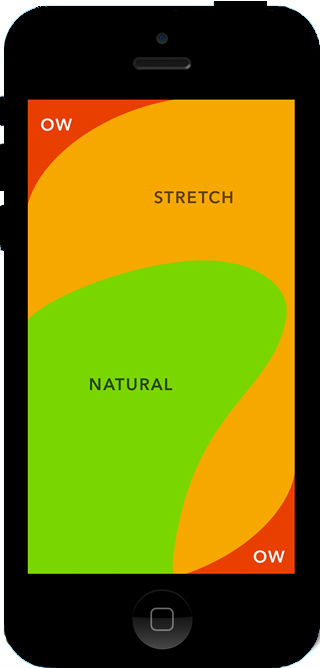
\includegraphics[scale=0.20]{pics/review/mobileScreen.jpg}
          \caption{The thumb zone}
          \label{fig:thumbZone}
        \end{figure}

      \subsection*{Experience with IT and security}

    \todo[inline, color=red!]{Need to describe which I selected and why}

	\subsection{Sampling Frame and Technique} \label{sec:sampling}
      
    The {\it sampling frame} is a list of the whole population of people that could be included in the survey. When looking at the sample of this study, there is not possible to make a limited sampling frame that can be summered in a list. The population of the sample frame is considered as all people with a smartphone.

    When conducting a survey, it needs to be decided how to select people from the sampling frame. There are two different ways of doing sampling: probability sampling and non-probability sampling \cite{empiriske}. Probability sampling means that the sample has been chosen because the researcher believes that there is a high probability that the sample of respondents selected is representative for the overall population being studied. Non-probability sampling means that the researcher does not know whether the sample of people is the overall population.

    Because of the broad sampling frame it would be feasible to use non-probability sampling for this research. When using non-probability sampling, we make a decision that it is not practicable to describe a representative sample because there is too much uncertainty about the respondents that will voluntary answer the questionnaire. When choosing a non-probability sampling, we need to select an {\it sampling technique}. The possible sampling techniques we can choose from is purposive sampling, snowball sampling, self-selection sampling, and convenience sampling. The {\it purposive sampling technique} requires the researcher deliberately to choose people that are likely to produce valuable data to meet the purpose of the research. This requirement would not be a good technique because I am not able to pick who would participate, as well as the data collection need to be performed worldwide. A Purposive sampling technique would maybe provide a more uniform collection of people, but it is hard to control respondents when the questionnaire is distributed on the Internet.
    The {\it snowball sampling technique} utilize the network from one person of the sample frame, and then collects new names from that person. The need for directly communicate with respondents is not possible for me as a researcher. {First}, I have no contact with the respondents. {Second}, the respondents, should remain anonymous when answering the questionnaire, as well as there should be possible to track the information back to the respondent.
    When using the {\it convenience sampling technique}, the researcher only select respondents who are convenient for them, because they are easy to reach or willing to help.

    When doing {\it self-selection sampling}, the researcher advertise their interest in a particular topic and their need for respondents, and collect data from anyone who are willing to participate. The self-selection sampling strategy looks like an excellent fit for the research. The questionnaire needs to be distributed over the Internet, and the self-selection strategy will support this choice. People who select themselves for research often do so because they have strong feeling for the subject, or that the research can bring them a personal benefit. A self-selection sampling technique may also reduce the bias that can be introduced when the researcher hand-picks the respondents. With the self-selection sampling strategy allows all interested peoples with a smartphone to participate in the research. The self-selection is a useful technique when we are not able to directly contact the potential respondents.

  \subsection{Calculating the Sample Size} \label{sec:samplesize}

    It is important to decide on an appropriate sample size in order to conclude that the results to be statistically significant. When a sample size is too big, it will lead to unnecessary waste of time in this study due to the time frame of this project. On the other hand, if the sample size is too small, the results will not be statistically significant, and it might not be possible to come up with a reliable conclusion.

    When looking a calculation of sample size you need to know the population size, preferred margin of error, desired confidence interval, and the percentage of the population that is likely to answer. In this study, these parameters are hard to determine because of the non-probability sampling that is selected for this study. Non-probability sampling refers to the selection of the sample that is based on unknown portability. It is distinguished from probability sampling by the fact that subjective judgments play a role in selecting the sampling size. When using non-probability sampling, it does not give a sample units an equal likelihood of being included in the sample. The sample units are chosen so they can represent the population, and is decided by the experience of the Researcher. Because of this uncertainty, there is not a known formula for calculating the sample size.

    We are not able to calculate the sample size by a known formula, but the sample size still needs to be decided based on my subjective meaning. The sample size is determined by what is achievable with the time frame available, as well as what I as a researcher think of as a good enough sample to ensure that the results can be statistically significant.

    One of the factors that were mentioned to be included when estimating the sample size was the targeted population size. When looking at the population size for this research, there is no good way to estimate that number because it includes all people with a smartphone worldwide.

    The greater the accuracy required by my claim that my sample size represent the whole population adequately; the larger your sample size needs to be. Statisticians have produced tables that correlate population size against the sample size required for the required level of confidence and accuracy. Researchers generally work with a confidence level of 95\% and an accuracy range of +/- 3 \%. In Table~\ref{tab:sampleSize} there is a recommended sample size for a survey (using 95\% confidence interval and +/- 3\% accuracy range) estimated by the targeted population size \cite{empiriske}.

    As we can see in Table~\ref{tab:sampleSize}, the sample size does not increase at the same rate as the target population. When looking at all people that owns a mobile phone worldwide, we can argue that the targeted population size is greater than 1,000,000, and we, therefore, need a sample size of at least 1000. It would be desirable to get a sample size bigger than 1000, but due to the time frame of this research, a sample size of 1000 would be good enough to get statistically significant results.

      \begin{table}[H]
      	\centering
        \begin{tabular}{| p{5cm} | p{5cm} |}
          \hline
          {\bf Target Population Size} & {\bf Required sample size} \\ \hline
          50 & 47 \\
          5000 & 760 \\ 
          100,000 & 888 \\
          900,000 & 895 \\ 
          $>$1,000,000 & 1000+ \\ \hline
        \end{tabular}
        \caption{Target population and sample size \cite{empiriske}}
        \label{tab:sampleSize}
      \end{table}

    Since the sampling size is quite hight, and the survey is going to be distributed with a self-selection sampling strategy over the Internet, it is still important to provide some level of control of the respondents. The lack of control of the respondents, there is likely to be some data properties that have a higher representation that others. Therefore, it is important to control the data collected during the spring. If it occurs that a subpopulation is overrepresented, it is desired to use the strategy for smoothing the data from Subsection. The data collected should never be manipulated. In a situation where there is lack of respondents from a subgroup, the only thing that I can do is to contact networks where there is a higher probability to reach the subgroup that is underrepresented in the sample. Of course, when using such a strategy, it might introduce some bias because I then influence the sample. Such an approach should only be used when there is lacking a number of respondents from a subgroup for getting statistically significant results. If using such a strategy, it should be highlighted in the results how I did it, as well as discuss how it might have impacted the results. 

    In the next section, we will look at some strategies for responses from different subgroups that may be underrepresented when using non-probability sampling with a self-selection technique. 

  \subsection{Response Rate and Non-responses} \label{sec:response}

    When sending out the questionnaire I have no control over how many people are willing to respond to the questionnaire or how many people from different subgroups I am able to reach. When talking about subgroups, it means that it is people with different human properties. To be able to achieve the amount of data needed for an analysis, I need to look for a strategy that may increase the number of responses from the different subgroups. If I suspect that certain types of people in my sample frame are less willing to respond or harder to reach, I could deliberately include more of that subgroup in my sample so I can assure that I receive the number of respondents that I need. Maybe go face-to-face if a particular group of people may be less willing to participate.

    In this list, there will be made a strategy for collecting data from the different subgroups. {\it First}, some subgroups might be less willing to respond to the questionnaire. {\it Second}, some of the subgroups might be harder to reach because they are outside of my network.

    {\bf People with age of 50 or higher:} People with the age over 50 may not own a smartphone or may be hard to reach for other reasons. I need to find networks were there is a high representation of people with an age of 50 or higher. In Norway, there is a network called ``Seniorweb''. There is also a magazine called ``vi over 60'' that is a network that is highly represented with people with an age over 60. Both networks are possible to contact if there is a lack of respondents from this subgroup.

    {\bf People with a different field of interest than IT and security:} My own network is overrepresented by people with a profession in IT and security. I need to be able to find other networks to be able to reach out to other people with other professions. To reach out to people with other professions, it is a possibility to use the network from my family or directly contact a company. The university is a good start because of the high representation of different field of study.

    {\bf People with a reading orientation from right-to-left:} The primary reading orientation is from right-to-left, with the exception of some Arabic and Asian nationalities. My network does not include a high sample of people that have another reading and writing orientation than my own. To reach out to other nationalities, I can contact NTNU and ask for help to distribute my questionnaire to countries where NTNU have exchange programs. ``International section'' or other networks like ``ISFiT'' (International Student Festival in Trondheim).

    {\bf People living in a different country than Norway:} I need to get in touch with people from different nationalities in order to get diversity in the collected data. I will contact the International Section at my university to ask them to distribute my questionnaire to the exchange students at my university. I am also having a trip to Minnesota in USA in the following spring, and I will use my time there recruiting people to respond to my questionnaire. During this semester, I have been talking to researchers in other countries because of their interest in my research. Hopefully, they can provide help to distribute the questionnaire to their own networks. As stated earlier, ``ISFiT'' is an international student festival in Trondheim. There are people traveling from all around the world to Trondheim.

    {\bf People that are left-handed:} There is a significant higher percentage of people that are right-handed, meaning that there is a possibility of getting more responses from people that are right-handed. Selecting a strategy for this is hard because there is not a known official network for left-handed people. There is a possibility of using groups at Facebook like ``Left-Hander's Club'' or a website called ``Left-handers day''.

    When analyzing the collected data, I need to find subgroups that have responded and those who have not. This will be used to make a discussion of why it lacked responses from a particular subgroup. The reason this is important is because their non-response might be meaningful in its own right, or their lack of responses may have introduced bias in the data. This part is out of scope for this thesis, but need to be considered in the next phase of this research.

  \subsection{Ethical Considerations}
    